\documentclass[graphics]{beamer}
\usepackage[utf8]{inputenc}
\usepackage[french]{babel}
\usepackage{lmodern}
\usepackage{tcolorbox}
\usepackage{pgfpages}
\usepackage{graphicx}
\usepackage{mathdots}
\usepackage{subcaption}
\usepackage{xcolor}
\usepackage[export]{adjustbox}
\usepackage{appendixnumberbeamer}
\usepackage{stmaryrd} 
\usepackage{minted}
\usepackage{caption}
\usepackage{version}
\captionsetup[figure]{labelformat=empty}



\usetheme{Warsaw}
\usecolortheme{dolphin}

\title[Algorithme génétique]{Algorithme génétique}
\subtitle{Groupe 4}
\author[R. Ageron, T. De Coninck, P. Dufresne, T. Pellerin]{Romain Ageron, Tom De Coninck, Paul Dufresne, Thibaut Pellerin}
\titlegraphic{\centering
	
\includegraphics[scale=.08]{cs}
}
%\institute[]{\'CentraleSupélec}
\date{1 février 2021}
	\setbeamersize{text margin left=15pt}
	\setbeamersize{text margin right=15pt}


% pour supprimer les symboles de navigation
\setbeamertemplate{navigation symbols}{}
% \setbeamertemplate{footline}[frame number]
\setbeamertemplate{caption}{\raggedright\insertcaption\par}

\newcommand\blfootnote[1]{%
	\begingroup
	\renewcommand\thefootnote{}\footnote{#1}%
	\addtocounter{footnote}{-1}%
	\endgroup
}

\begin{document}

\begin{frame}
\titlepage
%\begin{center}
%	\includegraphics[height=0.5cm]{logoens.pdf}
%\end{center}
\end{frame}

\section{Problème du plasmide circulaire}
\subsection{Présentation}
\begin{frame}
	On dispose d'une chaîne de nucléotides (A,T,C,G).
	\begin{itemize}
		\item chaque dinucléotide (ex : "AT") doit avoir une certaine orientation dans l'espace 
		\item on veut trouver les orientations qui rendent la trajectoire associée à la séquence \textbf{circulaire}
		\item nos variables sont les orientations, les individus seront donc des tables d'orientations
		\item on dispose de mesures expérimentales, les orientations doivent rester dans un intervalle autour de ces mesures
	\end{itemize}
\end{frame}
\begin{frame}
	\begin{center}
		\begin{tabular}{ | c || c | c | c | }
			\hline
			Paires/orientations & Twist & Wedge & Direction \\ \hline
			$AA$ & 35.62 & 7.2 & -154 \\ \hline
			$AC$ & 34.4 & 1.1 & 143 \\ \hline
			$AG$ & 27.7 & 8.4 & 2 \\ \hline
			... & ... & ... & ... \\ \hline
		\end{tabular}
	\end{center}
	On peut réduire le nombre de variables en exploitant les symétries : $AG^{-1} = CT$ et $AG$ et $CT$ ont même Twist, Wedge et leurs Directions sont opposées : on a finalement \textbf{20 variables}.
\end{frame}

\subsection{Principe de l'algorithme génétique}

\begin{frame}
	Une algorithme génétique est une méthode d'\textbf{optimisation} qui s'inspire de la sélection naturelle.
	\begin{figure}[H]
		\centering
		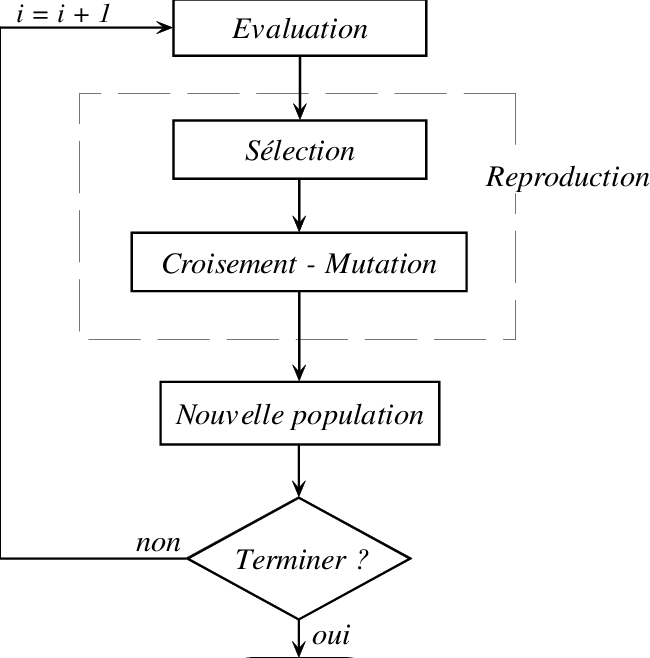
\includegraphics[scale=0.2]{algo_gen}
	\end{figure}
\end{frame}

\begin{frame}
	Les différentes étapes d'un algorithme génétique sont :
	\begin{itemize}
		\item \textbf{évaluation} : attribuer un score à un individu selon l'objectif du problème
		\item \textbf{sélection} : conserver certains individus via différentes méthodes (classement, tournoi...)
		\item \textbf{croisement} : créer de nouveaux individus à partir de ceux sélectionnés (permet de creuser un minimum)
		\item \textbf{mutation} : modifier aléatoirement certains individus (permet notamment de sortir d'un minimum local)
	\end{itemize}
\end{frame}

\section{Découpage du code}

\subsection{Méthode d'évaluation}

\begin{frame}
	\begin{figure}[H]
		\centering
		\begin{subfigure}[b]{0.4\textwidth}
			\centering
			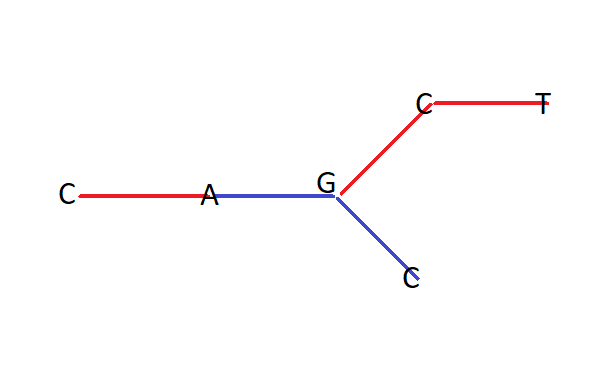
\includegraphics[width=\textwidth]{pb_angle}
			\caption{Bonne distance mais mauvaise orientation}
			\label{fig:y equals x}
		\end{subfigure}
		\begin{subfigure}[b]{0.4\textwidth}
			\centering
			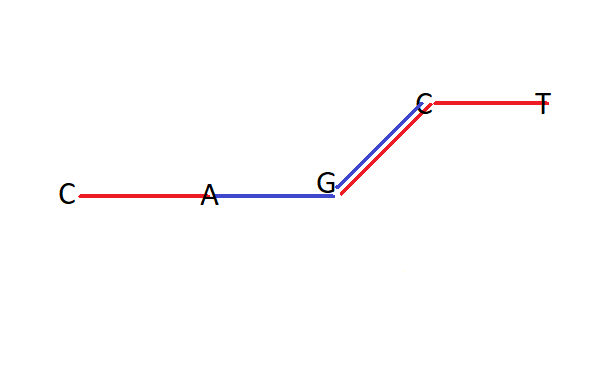
\includegraphics[width=\textwidth]{angle_oui}
			\caption{Bonne distance et bonne orientation}
			\label{fig:three sin x}
		\end{subfigure}
		\caption{Jonction pour une chaîne $GCT...CA$}
		\label{fig:three graphs}
	\end{figure}
Pour contrôler la qualité de la trajectoire, on ajoute (en bleu) les deux premiers nucléotides à la fin de la chaîne. Ici, $G$, le premier nucléotide, est bien placé mais l'orientation de $GC$ n'est pas forcément valide.
\end{frame}

\subsection{Classes} 

\begin{frame}

\begin{tabular}{| c |}
	\hline
	\mintinline{python}{AG} \\ \hline \hline
	\mintinline{python}{population} \\
	\mintinline{python}{pop_number}  \\ \hline
	\mintinline{python}{tournament} \\
	\mintinline{python}{reproduction} \\ \hline
\end{tabular}
\begin{tabular}{ | c | }
	\hline
	\mintinline{python}{Entity} \\ \hline \hline
	\mintinline{python}{param}  \\  
	\mintinline{python}{fitness}  \\ \hline
	\mintinline{python}{fitness_calculation} \\
	\mintinline{python}{mutation}  \\ \hline
\end{tabular}
\begin{tabular}{ | c | }
	\hline
	\mintinline{python}{RotTable} \\ \hline \hline
	\mintinline{python}{OriginalRotTable}  \\ 
	\mintinline{python}{interval}  \\ \hline
	\mintinline{python}{getTwist}  \\ 
	\mintinline{python}{rot_to_entity} \\ \hline
\end{tabular}
\vfill
Les deux premières classes sont génériques, et \mintinline{python}{RotTable} est propre au problème du plasmide circulaire. \mintinline{python}{AG} et \mintinline{python}{RotTable} font appel à \mintinline{python}{Entity}.
\end{frame}
\subsection{Quelques fonctions essentielles}

\begin{frame}
	Voici les fonctions qui correspondent aux différentes étapes de l'algorithme :
	\begin{itemize}
		\item la méthode \mintinline{python}{fitness_calculation} estime l'erreur de distance $d$ et d'orientation $o$, et renvoie $(1+d) \times (1+o)$
		\item pour la sélection, nous utilisons un tournoi probabiliste
		\item la reproduction est assez simple : dans un premier temps nous avons fait la moyenne de deux tables
		\item \mintinline{python}{mutation} modifie une des variables d'un individu 
		\item enfin, \mintinline{python}{global_mutation} fais muter une partie de la population 
	\end{itemize}
\end{frame}

\begin{frame}
	L'étape de mutation s'est révélée très importante :
	\begin{itemize}
		\item elle permet d'explorer l'espace du problème 
		\item des mutations trop limitées bloquent l'algorithme dans des minimums locaux
		\item des mutations excessives risquent de gâcher des individus prometteurs
	\end{itemize}
Nous avons choisi de faire muter une part importante de la population, mais pas les individus ayant les meilleurs scores. La mutation modifie une des variables, aléatoirement dans l'intervalle associé.
\end{frame}

\section{Résultats}
\subsection{Quelques images}

\begin{frame}
	La trajectoire totale est représentée à gauche, et la jonction à droite (un vecteur = un dinucléotide).
	\begin{figure}[H]
		\centering
		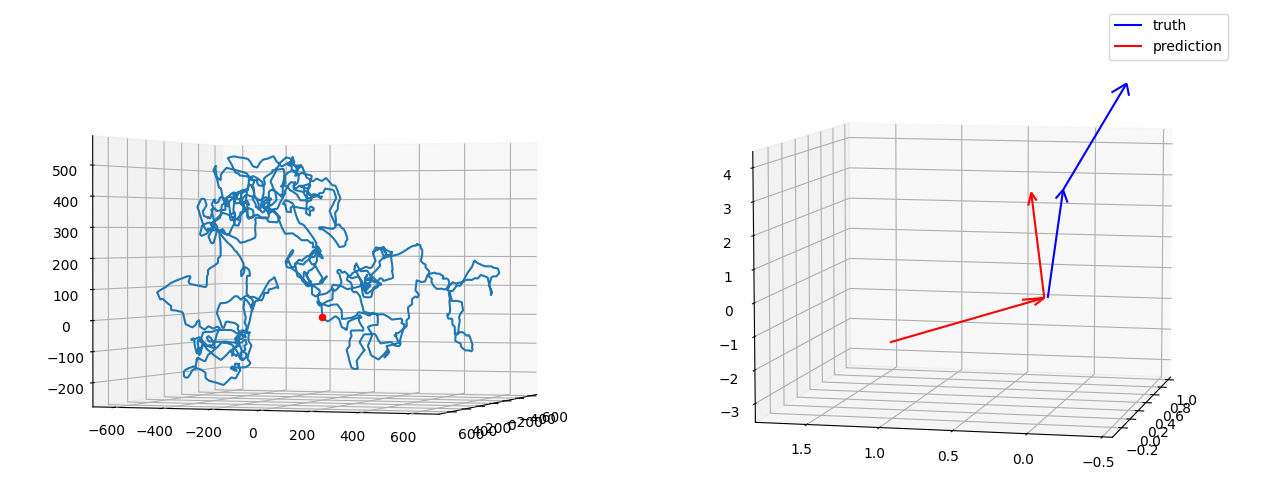
\includegraphics[scale=0.3]{8k_200gen_1000pop_tour0.3_mut0.7_1.038}
		\caption{Une chaîne de longueur 8000, avec 200 générations et une population de 1000}
	\end{figure}
	Ici, l'erreur de position est faible mais celle d'orientation non négligeable.
\end{frame}

\begin{frame}
	On peut modifier légèrement la fonction \mintinline{python}{fitness_calculation} afin de pénaliser davantage l'erreur sur l'angle.
	\begin{figure}[H]
		\centering
		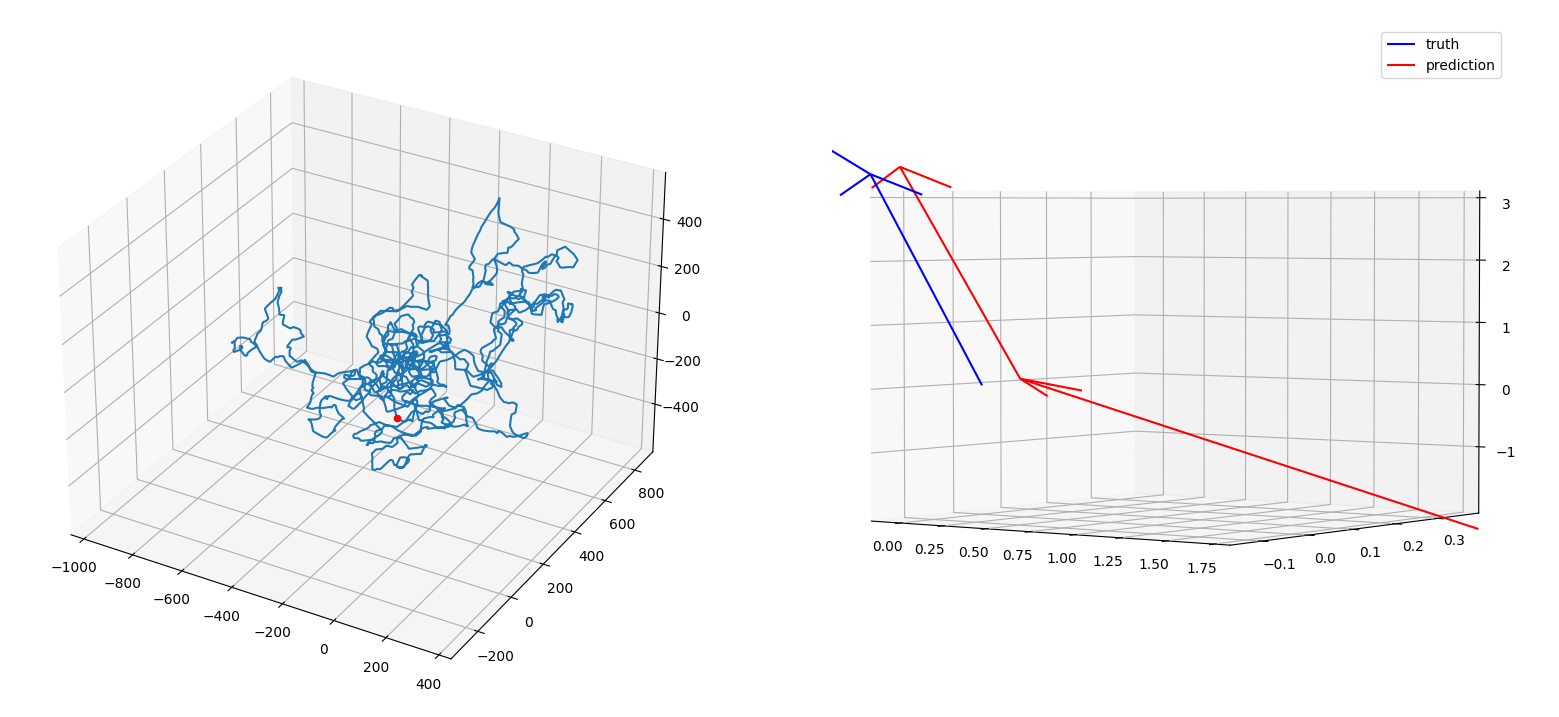
\includegraphics[scale=0.25]{250gen200pop0.3_0.003_0.7_0.003alpha=10}
		\caption{Une chaîne de longueur 8000, avec 250 générations et une population de 200}
	\end{figure}
	Les dinucléotides réel et fictif sont ici parallèles, mais la distance est plus importante.
\end{frame}

\begin{frame}
	Après une bonne heure de calcul, on obtient ceci pour une chaîne de 180000 nucléotides.
	\begin{figure}[H]
		\centering
		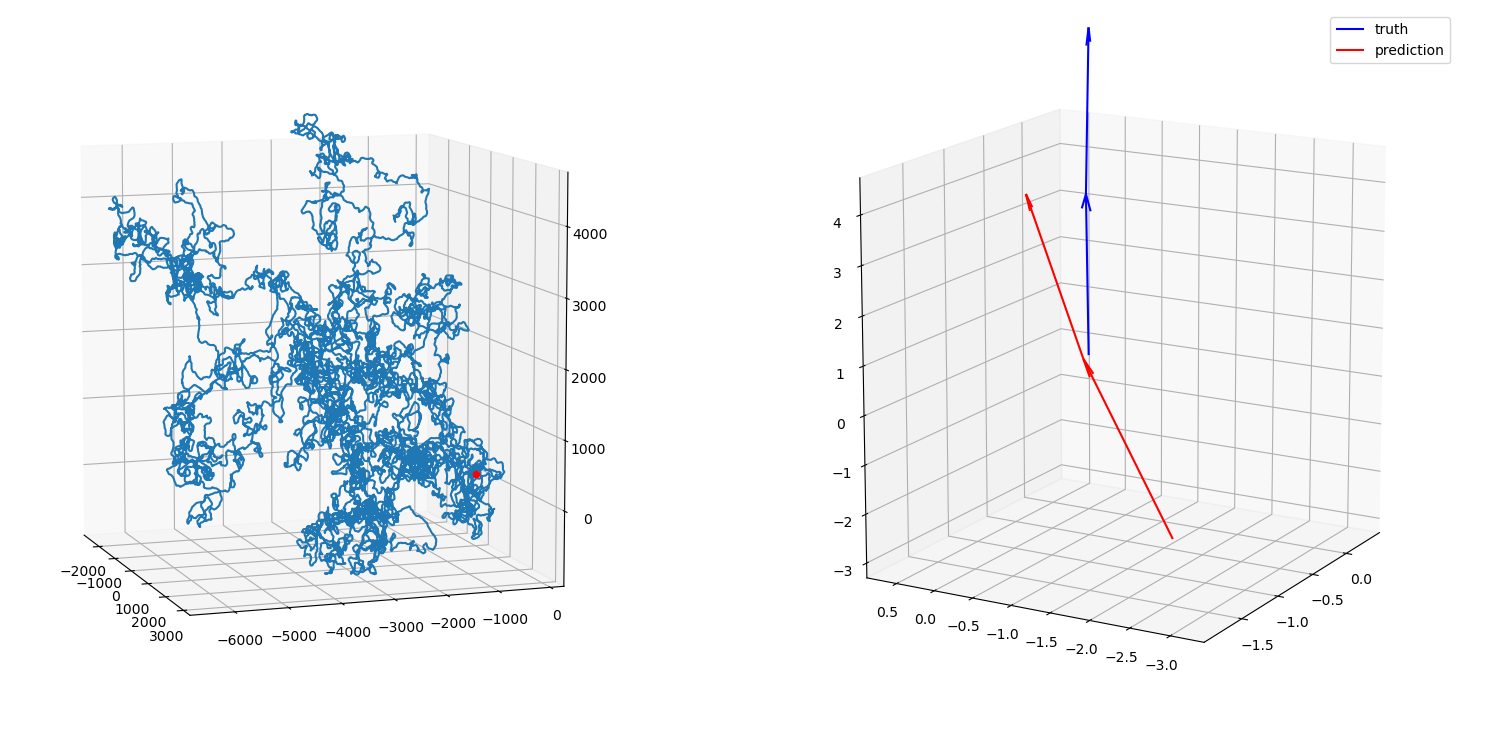
\includegraphics[scale=0.25]{180}
	\end{figure}
\end{frame}

\subsection{Commentaires}
	
\begin{frame}
	\begin{itemize}
		\item Le temps d'exécution est d'environ 3 minutes pour une chaîne de longueur 8000, une population de 100 et une centaine de générations
		\item L'accumulation d'erreurs numériques rend les résultats pour la chaîne de 180k peu fiables
		\item Difficile d'équilibrer la fonction \mintinline{python}{fitness_calculation} afin d'avoir une bonne distance et une bonne orientation
	\end{itemize}
\end{frame}

\subsection{Ouverture}

\begin{frame}
Ici, l'optimisation est \textbf{multi-critère}. Nous nous sommes ramené à une fonction \mintinline{python}{fitness_calculation} scalaire, mais il peut être plus efficace de mesurer indépendamment les deux erreurs. \\
On se prive alors de l'ordre sur $\mathbb{R}$, mais on peut pallier ce problème en utilisant par exemple des \textit{fronts de Pareto}.
\begin{figure}[H]
	\centering
	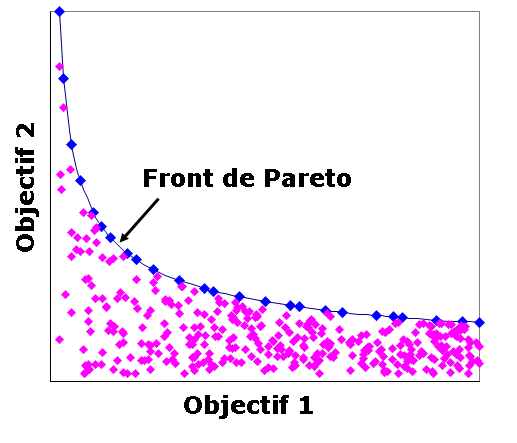
\includegraphics[scale=0.3]{pareto}
\end{figure}

Une autre idée serait de faire une fonction de mutation dynamique (par exemple plus de mutation lorsque l'algorithme stagne).
\end{frame}

\end{document}